\chapter{强关联效应导致的金属-绝缘体转变}\label{chap:interaction-transition}

\section{杂质导致的金属局域磁矩}

\subsection{Anderson杂质模型}\label{sec:anderson-model}

考虑一个无相互作用的体系,我们在其中引入一个杂质,并且假定该杂质能够将电子紧密地约束在其周围。
这样一来我们就有了两套能级:一套是原本的费米液体,还有一套是一个单独的能级,处于这个能级的电子被束缚在杂质周围。
需要使用晶格动量和自旋标记前者(仅考虑能量最低的能带),称为\concept{巡游电子},因为它的波函数是布洛赫波函数,并不定域;后者是定域的,只需要使用自旋即可标记后者,称为\concept{d电子}(因为很多时候这个轨道是杂质的d轨道)。
前者和后者可以自然地转化,即两者之间有\concept{杂化}。
于是描述它们的模型就是以下\concept{单杂质的Anderson模型}:
\begin{equation}
    {H} = \sum_{\vb*{k}, \sigma} (\epsilon_{\vb*{k}} - \mu) {c}_{\vb*{k}\sigma}^\dagger {c}_{\vb*{k} \sigma} + \sum_\sigma \epsilon_\text{d} {c}_{\text{d}\sigma}^\dagger {c}_{\text{d} \sigma} + \sum_{\vb*{k}, \sigma} V_{\vb*{k} \text{d}} {c}_{\vb*{k} \sigma}^\dagger {c}_{\text{d} \sigma} + \text{h.c.} + U {n}_{\text{d} \uparrow} {n}_{\text{d} \downarrow}.
    \label{eq:impurity-anderson}
\end{equation}
不失一般性地认为$V_{\vb*{k} \text{d}}$都是实数,如果它不是实数,那总是可以通过重新定义${c}_{\vb*{k} \text{d}}$(乘上一个复数因子)来让它变成实数。
最后一项是因为同处于d能级的两个电子之间会有库伦排斥作用,这一项实际上是唯一的真正的相互作用,因为前三项都是二次型。请注意这一项具有自选旋转不变性,这也是合理的。
与d轨道上的自旋-自旋排斥相比,巡游电子相互作用不会有显著的影响。

\begin{figure}
    \centering

    \tikzset{every picture/.style={line width=0.75pt}} %set default line width to 0.75pt        

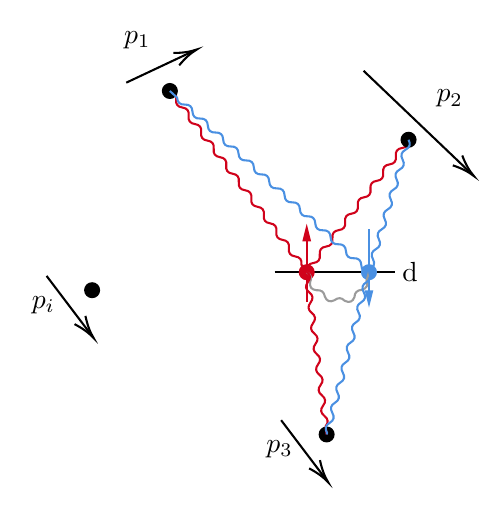
\begin{tikzpicture}[x=0.75pt,y=0.75pt,yscale=-1,xscale=1]
%uncomment if require: \path (0,235); %set diagram left start at 0, and has height of 235

%Straight Lines [id:da04263713787309409] 
\draw [color={rgb, 255:red, 74; green, 144; blue, 226 }  ,draw opacity=1 ]   (316.44,137.41) -- (316.44,101.71) ;
\draw [shift={(316.44,139.41)}, rotate = 270] [fill={rgb, 255:red, 74; green, 144; blue, 226 }  ,fill opacity=1 ][line width=0.08]  [draw opacity=0] (8.4,-2.1) -- (0,0) -- (8.4,2.1) -- cycle    ;
%Straight Lines [id:da10493507194641594] 
\draw [color={rgb, 255:red, 208; green, 2; blue, 27 }  ,draw opacity=1 ]   (286.44,136.69) -- (286.44,101) ;
\draw [shift={(286.44,99)}, rotate = 450] [fill={rgb, 255:red, 208; green, 2; blue, 27 }  ,fill opacity=1 ][line width=0.08]  [draw opacity=0] (8.4,-2.1) -- (0,0) -- (8.4,2.1) -- cycle    ;
%Straight Lines [id:da877105773313088] 
\draw [color={rgb, 255:red, 208; green, 2; blue, 27 }  ,draw opacity=1 ]   (220.5,35) .. controls (222.83,35.33) and (223.84,36.66) .. (223.52,38.99) .. controls (223.2,41.32) and (224.21,42.65) .. (226.54,42.97) .. controls (228.87,43.3) and (229.88,44.63) .. (229.56,46.96) .. controls (229.24,49.29) and (230.25,50.62) .. (232.58,50.94) .. controls (234.91,51.27) and (235.92,52.6) .. (235.59,54.93) .. controls (235.27,57.26) and (236.28,58.59) .. (238.61,58.91) .. controls (240.94,59.24) and (241.95,60.57) .. (241.63,62.9) .. controls (241.31,65.23) and (242.32,66.56) .. (244.65,66.89) .. controls (246.98,67.21) and (247.99,68.54) .. (247.67,70.87) .. controls (247.35,73.2) and (248.36,74.53) .. (250.69,74.86) .. controls (253.02,75.18) and (254.03,76.51) .. (253.71,78.84) .. controls (253.39,81.17) and (254.4,82.5) .. (256.73,82.83) .. controls (259.06,83.15) and (260.07,84.48) .. (259.75,86.81) .. controls (259.43,89.14) and (260.44,90.47) .. (262.77,90.8) .. controls (265.1,91.13) and (266.11,92.46) .. (265.78,94.79) .. controls (265.46,97.12) and (266.47,98.45) .. (268.8,98.77) .. controls (271.13,99.1) and (272.14,100.43) .. (271.82,102.76) .. controls (271.5,105.09) and (272.51,106.42) .. (274.84,106.74) .. controls (277.17,107.07) and (278.18,108.4) .. (277.86,110.73) .. controls (277.54,113.06) and (278.55,114.39) .. (280.88,114.71) .. controls (283.21,115.04) and (284.22,116.37) .. (283.9,118.7) -- (286.44,122.06) -- (286.44,122.06) ;
%Straight Lines [id:da42896076161061414] 
\draw [color={rgb, 255:red, 208; green, 2; blue, 27 }  ,draw opacity=1 ]   (335.5,58.5) .. controls (335.81,60.84) and (334.79,62.16) .. (332.45,62.46) .. controls (330.11,62.76) and (329.09,64.08) .. (329.39,66.42) .. controls (329.69,68.75) and (328.67,70.07) .. (326.34,70.37) .. controls (324,70.67) and (322.98,71.99) .. (323.28,74.33) .. controls (323.59,76.67) and (322.57,77.99) .. (320.23,78.29) .. controls (317.89,78.59) and (316.87,79.91) .. (317.17,82.25) .. controls (317.48,84.59) and (316.46,85.91) .. (314.12,86.21) .. controls (311.78,86.51) and (310.76,87.83) .. (311.06,90.17) .. controls (311.36,92.5) and (310.34,93.82) .. (308.01,94.12) .. controls (305.67,94.42) and (304.65,95.74) .. (304.95,98.08) .. controls (305.26,100.42) and (304.24,101.74) .. (301.9,102.04) .. controls (299.56,102.34) and (298.54,103.66) .. (298.84,106) .. controls (299.15,108.34) and (298.13,109.66) .. (295.79,109.96) .. controls (293.45,110.26) and (292.43,111.58) .. (292.73,113.92) .. controls (293.03,116.25) and (292.01,117.57) .. (289.68,117.87) .. controls (287.34,118.17) and (286.32,119.49) .. (286.62,121.83) -- (286.44,122.06) -- (286.44,122.06) ;
%Straight Lines [id:da4767709807473357] 
\draw    (271,122) -- (329,122) ;
%Straight Lines [id:da756549749402925] 
\draw    (199.5,31) -- (231.69,15.85) ;
\draw [shift={(233.5,15)}, rotate = 514.8] [color={rgb, 255:red, 0; green, 0; blue, 0 }  ][line width=0.75]    (10.93,-3.29) .. controls (6.95,-1.4) and (3.31,-0.3) .. (0,0) .. controls (3.31,0.3) and (6.95,1.4) .. (10.93,3.29)   ;
%Straight Lines [id:da5187366946219611] 
\draw    (220.5,35) ;
\draw [shift={(220.5,35)}, rotate = 0] [color={rgb, 255:red, 0; green, 0; blue, 0 }  ][fill={rgb, 255:red, 0; green, 0; blue, 0 }  ][line width=0.75]      (0, 0) circle [x radius= 3.35, y radius= 3.35]   ;

%Straight Lines [id:da940330546706269] 
\draw    (274.11,193.61) -- (295.59,221.97) ;
\draw [shift={(296.8,223.56)}, rotate = 232.86] [color={rgb, 255:red, 0; green, 0; blue, 0 }  ][line width=0.75]    (10.93,-3.29) .. controls (6.95,-1.4) and (3.31,-0.3) .. (0,0) .. controls (3.31,0.3) and (6.95,1.4) .. (10.93,3.29)   ;
%Straight Lines [id:da21455240162669864] 
\draw    (296.04,200.48) ;
\draw [shift={(296.04,200.48)}, rotate = 0] [color={rgb, 255:red, 0; green, 0; blue, 0 }  ][fill={rgb, 255:red, 0; green, 0; blue, 0 }  ][line width=0.75]      (0, 0) circle [x radius= 3.35, y radius= 3.35]   ;
%Straight Lines [id:da9480520110643911] 
\draw    (313.85,25.29) -- (365.55,74.62) ;
\draw [shift={(367,76)}, rotate = 223.66] [color={rgb, 255:red, 0; green, 0; blue, 0 }  ][line width=0.75]    (10.93,-3.29) .. controls (6.95,-1.4) and (3.31,-0.3) .. (0,0) .. controls (3.31,0.3) and (6.95,1.4) .. (10.93,3.29)   ;
%Straight Lines [id:da36481378083827076] 
\draw    (335.5,58.5) ;
\draw [shift={(335.5,58.5)}, rotate = 0] [color={rgb, 255:red, 0; green, 0; blue, 0 }  ][fill={rgb, 255:red, 0; green, 0; blue, 0 }  ][line width=0.75]      (0, 0) circle [x radius= 3.35, y radius= 3.35]   ;
%Straight Lines [id:da8628136716727641] 
\draw [color={rgb, 255:red, 208; green, 2; blue, 27 }  ,draw opacity=1 ]   (286.44,122.31) ;
\draw [shift={(286.44,122.31)}, rotate = 0] [color={rgb, 255:red, 208; green, 2; blue, 27 }  ,draw opacity=1 ][fill={rgb, 255:red, 208; green, 2; blue, 27 }  ,fill opacity=1 ][line width=0.75]      (0, 0) circle [x radius= 3.35, y radius= 3.35]   ;
%Straight Lines [id:da5070042296264563] 
\draw [color={rgb, 255:red, 74; green, 144; blue, 226 }  ,draw opacity=1 ]   (316.44,122.31) ;
\draw [shift={(316.44,122.31)}, rotate = 0] [color={rgb, 255:red, 74; green, 144; blue, 226 }  ,draw opacity=1 ][fill={rgb, 255:red, 74; green, 144; blue, 226 }  ,fill opacity=1 ][line width=0.75]      (0, 0) circle [x radius= 3.35, y radius= 3.35]   ;
%Straight Lines [id:da46289377926067] 
\draw [color={rgb, 255:red, 74; green, 144; blue, 226 }  ,draw opacity=1 ]   (335.5,58.5) .. controls (336.62,60.57) and (336.14,62.17) .. (334.07,63.29) .. controls (332,64.41) and (331.52,66.01) .. (332.64,68.08) .. controls (333.76,70.15) and (333.28,71.75) .. (331.21,72.87) .. controls (329.14,73.99) and (328.66,75.59) .. (329.78,77.66) .. controls (330.9,79.73) and (330.42,81.33) .. (328.35,82.45) .. controls (326.28,83.58) and (325.8,85.18) .. (326.92,87.25) .. controls (328.04,89.32) and (327.56,90.92) .. (325.49,92.04) .. controls (323.42,93.16) and (322.94,94.76) .. (324.05,96.83) .. controls (325.17,98.9) and (324.69,100.5) .. (322.62,101.62) .. controls (320.55,102.74) and (320.07,104.34) .. (321.19,106.41) .. controls (322.31,108.48) and (321.83,110.08) .. (319.76,111.2) .. controls (317.69,112.32) and (317.21,113.92) .. (318.33,115.99) .. controls (319.45,118.06) and (318.97,119.66) .. (316.9,120.78) -- (316.44,122.31) -- (316.44,122.31) ;
%Straight Lines [id:da8075589571416464] 
\draw [color={rgb, 255:red, 74; green, 144; blue, 226 }  ,draw opacity=1 ]   (316.44,122.31) .. controls (314.09,122.42) and (312.86,121.3) .. (312.75,118.95) .. controls (312.64,116.6) and (311.4,115.47) .. (309.05,115.58) .. controls (306.7,115.69) and (305.46,114.57) .. (305.35,112.22) .. controls (305.24,109.87) and (304,108.74) .. (301.65,108.85) .. controls (299.3,108.96) and (298.06,107.84) .. (297.95,105.49) .. controls (297.84,103.14) and (296.61,102.01) .. (294.26,102.12) .. controls (291.91,102.23) and (290.67,101.1) .. (290.56,98.75) .. controls (290.45,96.4) and (289.21,95.28) .. (286.86,95.39) .. controls (284.51,95.5) and (283.27,94.37) .. (283.16,92.02) .. controls (283.05,89.67) and (281.81,88.55) .. (279.46,88.66) .. controls (277.11,88.77) and (275.88,87.64) .. (275.77,85.29) .. controls (275.66,82.94) and (274.42,81.82) .. (272.07,81.93) .. controls (269.72,82.04) and (268.48,80.91) .. (268.37,78.56) .. controls (268.26,76.21) and (267.02,75.09) .. (264.67,75.2) .. controls (262.32,75.31) and (261.08,74.18) .. (260.97,71.83) .. controls (260.86,69.48) and (259.63,68.36) .. (257.28,68.47) .. controls (254.93,68.58) and (253.69,67.45) .. (253.58,65.1) .. controls (253.47,62.75) and (252.23,61.63) .. (249.88,61.74) .. controls (247.53,61.85) and (246.29,60.72) .. (246.18,58.37) .. controls (246.07,56.02) and (244.83,54.9) .. (242.48,55.01) .. controls (240.13,55.12) and (238.9,53.99) .. (238.79,51.64) .. controls (238.68,49.29) and (237.44,48.17) .. (235.09,48.28) .. controls (232.74,48.39) and (231.5,47.26) .. (231.39,44.91) .. controls (231.28,42.56) and (230.04,41.44) .. (227.69,41.55) .. controls (225.34,41.66) and (224.1,40.53) .. (223.99,38.18) -- (220.5,35) -- (220.5,35) ;
%Curve Lines [id:da513294333685683] 
\draw [color={rgb, 255:red, 155; green, 155; blue, 155 }  ,draw opacity=1 ]   (286.44,122.31) .. controls (288.45,123.42) and (289.01,125) .. (288.12,127.05) .. controls (287.71,129.44) and (288.72,130.76) .. (291.15,130.99) .. controls (293.43,130.76) and (294.77,131.77) .. (295.17,134.02) .. controls (296.06,136.29) and (297.59,136.89) .. (299.77,135.83) .. controls (301.57,134.4) and (303.22,134.49) .. (304.73,136.08) .. controls (307,137.21) and (308.57,136.62) .. (309.44,134.31) .. controls (309.51,132.12) and (310.7,130.95) .. (312.99,130.81) .. controls (315.38,130.05) and (316.13,128.59) .. (315.26,126.42) -- (316.44,122.31) ;
%Straight Lines [id:da13970681970843724] 
\draw [color={rgb, 255:red, 208; green, 2; blue, 27 }  ,draw opacity=1 ]   (286.44,122.06) .. controls (288.3,123.51) and (288.5,125.17) .. (287.05,127.02) .. controls (285.6,128.88) and (285.8,130.54) .. (287.66,131.99) .. controls (289.52,133.44) and (289.72,135.09) .. (288.27,136.95) .. controls (286.82,138.8) and (287.02,140.46) .. (288.87,141.91) .. controls (290.73,143.36) and (290.93,145.02) .. (289.48,146.88) .. controls (288.03,148.74) and (288.23,150.39) .. (290.09,151.84) .. controls (291.95,153.29) and (292.15,154.94) .. (290.7,156.8) .. controls (289.25,158.65) and (289.45,160.31) .. (291.3,161.77) .. controls (293.16,163.22) and (293.36,164.87) .. (291.91,166.73) .. controls (290.46,168.59) and (290.66,170.24) .. (292.52,171.69) .. controls (294.38,173.14) and (294.58,174.79) .. (293.13,176.65) .. controls (291.68,178.5) and (291.88,180.16) .. (293.73,181.62) .. controls (295.59,183.07) and (295.79,184.72) .. (294.34,186.58) .. controls (292.89,188.44) and (293.09,190.09) .. (294.95,191.54) .. controls (296.81,192.99) and (297.01,194.65) .. (295.56,196.51) -- (296.04,200.48) -- (296.04,200.48) ;
%Straight Lines [id:da06596795786329368] 
\draw [color={rgb, 255:red, 74; green, 144; blue, 226 }  ,draw opacity=1 ]   (316.44,122.31) .. controls (317.63,124.34) and (317.21,125.96) .. (315.18,127.15) .. controls (313.15,128.34) and (312.73,129.96) .. (313.92,131.99) .. controls (315.11,134.02) and (314.69,135.64) .. (312.66,136.83) .. controls (310.63,138.02) and (310.2,139.63) .. (311.39,141.66) .. controls (312.58,143.69) and (312.16,145.31) .. (310.13,146.5) .. controls (308.1,147.69) and (307.68,149.31) .. (308.87,151.34) .. controls (310.06,153.37) and (309.64,154.99) .. (307.61,156.18) .. controls (305.58,157.37) and (305.15,158.99) .. (306.34,161.02) .. controls (307.53,163.05) and (307.11,164.66) .. (305.08,165.85) .. controls (303.05,167.04) and (302.63,168.66) .. (303.82,170.69) .. controls (305.01,172.72) and (304.59,174.34) .. (302.56,175.53) .. controls (300.53,176.72) and (300.1,178.34) .. (301.29,180.37) .. controls (302.48,182.4) and (302.06,184.02) .. (300.03,185.21) .. controls (298,186.4) and (297.58,188.01) .. (298.77,190.04) .. controls (299.96,192.07) and (299.54,193.69) .. (297.51,194.88) .. controls (295.48,196.07) and (295.05,197.69) .. (296.24,199.72) -- (296.04,200.48) -- (296.04,200.48) ;
%Straight Lines [id:da8698616226758178] 
\draw    (161.11,124.11) -- (182.59,152.47) ;
\draw [shift={(183.8,154.06)}, rotate = 232.86] [color={rgb, 255:red, 0; green, 0; blue, 0 }  ][line width=0.75]    (10.93,-3.29) .. controls (6.95,-1.4) and (3.31,-0.3) .. (0,0) .. controls (3.31,0.3) and (6.95,1.4) .. (10.93,3.29)   ;
%Straight Lines [id:da75441343254533] 
\draw    (183.04,130.98) ;
\draw [shift={(183.04,130.98)}, rotate = 0] [color={rgb, 255:red, 0; green, 0; blue, 0 }  ][fill={rgb, 255:red, 0; green, 0; blue, 0 }  ][line width=0.75]      (0, 0) circle [x radius= 3.35, y radius= 3.35]   ;

% Text Node
\draw (331,122) node [anchor=west] [inner sep=0.75pt]   [align=left] {d};
% Text Node
\draw (197,5) node [anchor=north west][inner sep=0.75pt]    {$\boldsymbol{p}_{1}$};
% Text Node
\draw (347.5,33) node [anchor=north west][inner sep=0.75pt]    {$\boldsymbol{p}_{2}$};
% Text Node
\draw (265.5,202) node [anchor=north west][inner sep=0.75pt]    {$\boldsymbol{p}_{3}$};
% Text Node
\draw (152.5,132.5) node [anchor=north west][inner sep=0.75pt]    {$\boldsymbol{p}_{i}$};

\end{tikzpicture}

    \caption{Anderson模型,d电子可以和巡游电子相互转换(使用红色和蓝色的波浪线表示),不同自旋的d电子相互排斥(灰色波浪线)}
    \label{fig:anderson-model}
\end{figure}

d电子的相互作用项意味着d轨道上出现两个电子会大大增大能量,如果费米面位于d轨道出现一个电子和d轨道出现两个电子的能量之间,那么巡游电子总会填充d轨道,而且填充一个电子,其结果就是产生杂质附近的局域磁矩。
实际上,这样会导致一个低能有效理论,见\autoref{sec:kondo-effect}。
本节则主要观察什么时候会出现一个局域磁矩,即什么时候会出现对称性自发破缺。

在展开计算之前,首先尝试做一些定性的分析。记能谱展宽为$\Delta$,则由费米黄金法则,
\[
    \Delta \propto \frac{1}{\tau} \propto \sum_{\vb*{k}} \abs{V_{\vb*{k} \text{d}}}^2 N(\epsilon_\text{d}).
\]
只有$U$很大时才能够产生局域磁矩,否则d轨道可以很容易地填满。
当$U \gg \epsilon_\text{d} \gg \Delta$时,d电子能谱发生弱展宽,但仍然有清晰的能级,并且会有一个良定义的局域磁矩。
而当$U \gg \Delta \gg \epsilon_\text{d}$时能级已经很不清楚,d电子可以和费米海中大范围的电子发生相互作用,因此虽然d轨道上只有一个电子,但它会频繁地发生自旋翻转,因此不会有局域磁矩。

\subsection{平均场近似}

相互作用项为
\[
    U {n}_{\text{d} \uparrow} {n}_{\text{d} \downarrow} = U {c}_{\text{d} \uparrow}^\dagger {c}_{\text{d} \uparrow} {c}^\dagger_{\text{d} \downarrow} {c}_{\text{d} \downarrow},
\]
现在尝试应用平均场近似。假定体系近似自由,我们有
\[
    \begin{aligned}
        \expval{U {n}_{\text{d} \uparrow} {n}_{\text{d} \downarrow}} &= U \expval*{{c}_{\text{d} \uparrow}^\dagger {c}_{\text{d} \uparrow} {c}^\dagger_{\text{d} \downarrow} {c}_{\text{d} \downarrow}} \\
        &= U ( \expval*{{c}_{\text{d} \uparrow}^\dagger {c}_{\text{d} \uparrow}} \expval*{{c}_{\text{d} \downarrow}^\dagger {c}_{\text{d} \downarrow}} + \expval*{{c}_{\text{d} \uparrow}^\dagger {c}_{\text{d} \downarrow}} \expval*{{c}_{\text{d} \uparrow} {c}^\dagger_{\text{d} \downarrow}} ),
    \end{aligned}
\]
第二项如果有非零值,$z$方向上的自旋旋转对称性就破缺了。
确实有这样的可能,就是系统基态有对称性自发破缺,但这里暂时假定没有这种情况。%
\footnote{从这里也可以看到平均场近似总是倾向于高估系统的对称性破缺,因为我们完全可以假定$z$方向上的自旋旋转对称性真的破缺了,从而得到一个$z$方向上自选旋转对称性真的破缺的平均场理论。
}%
这样就有
\[
    \expval{U {n}_{\text{d} \uparrow} {n}_{\text{d} \downarrow}} = U \expval*{{c}_{\text{d} \uparrow}^\dagger {c}_{\text{d} \uparrow}} \expval*{{c}_{\text{d} \downarrow}^\dagger {c}_{\text{d} \downarrow}},
\]
这又告诉我们,我们有
\[
    \expval{U {n}_{\text{d} \uparrow} {n}_{\text{d} \downarrow}} = \expval{ U {n}_{\text{d} \uparrow} \expval*{{n}_{\text{d} \downarrow}} + U \expval*{{n}_{\text{d} \uparrow}} {n}_{\text{d} \downarrow} - U \expval*{{n}_{\text{d} \uparrow}} \expval*{{n}_{\text{d} \downarrow}} },
\]
那么如果相互作用哈密顿量适用平均场近似我们就有
\begin{equation}
    U {n}_{\text{d} \uparrow} {n}_{\text{d} \downarrow} \approx U {n}_{\text{d} \uparrow} \expval*{{n}_{\text{d} \downarrow}} + U \expval*{{n}_{\text{d} \uparrow}} {n}_{\text{d} \downarrow} - U \expval*{{n}_{\text{d} \uparrow}} \expval*{{n}_{\text{d} \downarrow}}.
\end{equation}
当然,这只是一种可能的平均场分解——没有理由认为这就是最理想的近似,但实际上使用变分计算可以确定这确实是最理想的近似。
忽略仅改变能量零点的常数项,得到平均场哈密顿量
\begin{equation}
    {H}_\text{MF} = \sum_{\vb*{k}, \sigma} \xi_{\vb*{k}} {c}_{\vb*{k}\sigma}^\dagger {c}_{\vb*{k} \sigma} + \sum_\sigma \epsilon_\text{d} {c}_{\text{d}\sigma}^\dagger {c}_{\text{d} \sigma} + \sum_{\vb*{k}, \sigma} V_{\vb*{k} \text{d}} {c}_{\vb*{k} \sigma}^\dagger {c}_{\text{d} \sigma} + \text{h.c.} + U {n}_{\text{d} \uparrow} \expval*{{n}_{\text{d} \downarrow}} + U \expval*{{n}_{\text{d} \uparrow}} {n}_{\text{d} \downarrow}.
    \label{eq:anderson-mf}
\end{equation}
这是一个二次型哈密顿量。\eqref{eq:anderson-mf}含有不确定的参数$\expval*{{n}_{\text{d} \uparrow}}$和$\expval*{{n}_{\text{d} \downarrow}}$(这两个参数实际上是序参量,它们的差给出了$z$轴上的磁矩),但是可以将它们当成参数,求解出${n}_{\text{d} \uparrow}$和${n}_{\text{d} \downarrow}$之后回代,从而形成自洽方程。

求解\eqref{eq:anderson-mf},在适当的条件上我们会看到$\expval*{{n}_{\text{d} \uparrow}} - \expval*{{n}_{\text{d} \downarrow}}$不等于零,即出现了一个自发磁矩。
虽然出现了一个局域磁矩,但这和我们的假定——$z$方向上自选旋转不变——并不矛盾,因为$z$方向上的自旋破缺的是$x$或$y$方向的自旋旋转不变性。
换而言之,以上我们证明的结论是:平均场理论下,$x, y, z$三个方向上的自选旋转不变性不可能全部保留,保留$z$轴的自旋旋转不变性就必定破坏其它两个方向的自选旋转不变性。

可以对\eqref{eq:anderson-mf}做对角化。定义
\begin{equation}
    E_{\text{d} \sigma} = \epsilon_\text{d} + U \expval*{{n}_{\text{d} (-\sigma)}},
    \label{eq:energy-d-sigma}
\end{equation}
则
\begin{equation}
    {H}_\text{MF} = \sum_{\vb*{k}, \sigma} \xi_{\vb*{k}} {c}_{\vb*{k}\sigma}^\dagger {c}_{\vb*{k} \sigma} + \sum_\sigma E_{\text{d} \sigma} {c}_{\text{d}\sigma}^\dagger {c}_{\text{d} \sigma} + \sum_{\vb*{k}, \sigma} V_{\vb*{k} \text{d}} {c}_{\vb*{k} \sigma}^\dagger {c}_{\text{d} \sigma} + \text{h.c.}
\end{equation}
下面要对角化该哈密顿量。设已有对角化形式
\[
    {H}_\text{MF} = \sum_{n, \sigma} \epsilon_{n \sigma} {c}^\dagger_{n\sigma} {c}_{n\sigma},
\]
其中$n$是某个未知的量子数,${c}_{n \sigma}$可以写成${c}_{\vb*{k} \sigma}$和${c}_{\text{d} \sigma}$的幺正变换,通过要求对易关系一致(或者别的什么技巧)就得到方程组
\begin{equation}
    \begin{aligned}
        \epsilon_{n\sigma} \braket{\vb*{k}\sigma}{n \sigma} &= \braket{\vb*{k} \sigma}{n \sigma} \xi_{\vb*{k}} + \braket{\text{d} \sigma}{n \sigma} V_{\vb*{k} \text{d}}, \\
        \epsilon_{n \sigma} \braket{\text{d} \sigma}{n \sigma} &= \braket{\text{d} \sigma}{n \sigma} E_{\text{d} \sigma} + \sum_{\vb*{k}} \braket{\vb*{k} \sigma}{n \sigma} V_{\vb*{k} \sigma}.
    \end{aligned}
\end{equation}
求解此方程组,并加入幺正性条件,就可以完成对角化。

\subsection{平均场近似下的格林函数}

由于系统自旋守恒,两个自旋不同的算符的格林函数为零,因此可以使用$G_{\text{dd}, \sigma}$标记d轨道电子的格林函数,用$G_{\vb*{k} \text{d}, \sigma}$标记从$\vb*{k}$动量的巡游电子跃迁为d电子的格林函数。
从一个巡游电子到另一个巡游电子的过程动量守恒(因为相当于积掉了d电子自由度),用$G_{\vb*{k}\sigma}$标记这个过程的格林函数。
我们并不会计算这些格林函数,于是首先考虑$n$-$\sigma$表象下的格林函数,然后再使用表象变换得到d电子或者别的什么东西的格林函数。
要计算d点子格林函数是为了计算$\expval*{{n}_{\text{d}\uparrow}}$和$\expval*{{n}_{\text{d}\downarrow}}$。

在$n$-$\sigma$表象下哈密顿量对角,于是使用$G_{n\sigma}$标记$n$表象电子的格林函数。
首先考虑松原格林函数,考虑到$n$表象下系统是自由的,有
\begin{equation}
    G_{n\sigma} (\omega_n) = \frac{1}{\ii \omega_n - \epsilon_n},
\end{equation}
请注意这里有两种$n$:$\omega_n$中的$n$标记频率,$\epsilon_n$和$G$的下标中的$n$则是量子数。
虚频单电子格林算符定义为
\[
    (\ii \omega_n - {h}_\text{MF}) {G}(\omega_n) = 1,
\]
使用$G_{n \sigma}$,单电子格林算符就是
\begin{equation}
    {G}(\omega_n) = \sum_{n, \sigma} \frac{\dyad{n\sigma}}{\ii \omega_n - \epsilon_n} = \frac{1}{\ii \omega_n - {h}_\text{MF}},
\end{equation}
其中${h}_\text{MF}$就是单体哈密顿量,为
\begin{equation}
    {h}_\text{MF} = \sum_{\vb*{k}, \sigma} \xi_{\vb*{k}} \dyad{\vb*{k} \sigma} + \sum_\sigma E_{\text{d} \sigma} \dyad{\text{d} \sigma} + \sum_{\vb*{k}, \sigma} V_{\vb*{k} \text{d}} ( \ket{\vb*{k} \sigma} \bra{\text{d} \sigma} + \text{h.c.} ).
    \label{eq:anderson-green-operator}
\end{equation}
格林算符在不同表象下的矩阵元就给出了全部的单电子格林函数(或者说二算符格林函数)。

计算\eqref{eq:anderson-green-operator}在$\vb*{k}, \text{d}$表象下的不同矩阵元,可以得到$G_{\text{dd}, \sigma}$,$G_{\vb*{k} \text{d}, \sigma}$和$G_{\vb*{k}, \sigma}$之间的关系。
可以预期$G_{\vb*{k}, \sigma}$和自由情况不会差太多,因为巡游电子远远多于d电子。
d电子的格林函数相对自由电子格林函数则会有较大的修正,具体而言,是
\begin{equation}
    (G_{\text{dd}, \sigma}(\omega_n))^{-1} = \ii \omega_n - E_{\text{d}\sigma} - \sum_{\vb*{k}} \frac{V_{\vb*{k}\text{d}}^2}{\ii \omega_n - \epsilon_{\vb*{k}}}.
\end{equation}
相应的推迟格林函数是
\begin{equation}
    (G_{\text{dd}, \sigma}^\text{ret}(\omega))^{-1} = \omega - E_{\text{d}\sigma} - \sum_{\vb*{k}} \frac{V_{\vb*{k}\text{d}}^2}{\omega - \epsilon_{\vb*{k}} + \ii 0^+}.
\end{equation}
自能修正为
\begin{equation}
    \Sigma_{\text{d} \sigma}^\text{ret} = \sum_{\vb*{k}} \frac{V_{\vb*{k}\text{d}}^2}{\omega - \epsilon_{\vb*{k}} + \ii 0^+} = \frac{V}{(2\pi)^3} \int \dd[3]{\vb*{k}} \frac{V_{\vb*{k}\text{d}}^2}{\omega - \epsilon_{\vb*{k}} + \ii 0^+}.
\end{equation}
它来自d电子通过和巡游电子作用,间接地“自己和自己相互作用”。它的实部带来能级修正,它的虚部就是能级展宽的量级。
实部是通常的柯西积分主值
\[
    \Re \Sigma_{\text{d} \sigma}^\text{ret} = \frac{V}{(2\pi)^3} \primevalue \int \dd[3]{\vb*{k}} \frac{V_{\vb*{k}\text{d}}^2}{\omega - \epsilon_{\vb*{k}} + \ii 0^+},
\]
虚部为
\[
    \Im \Sigma_{\text{d} \sigma}^\text{ret} = - \frac{V}{(2\pi)^3} \int \dd[3]{\vb*{k}} \pi \delta(\omega - \epsilon_{\vb*{k}}) V_{\vb*{k} \text{d}}^2 .
\]
我们在费米面附近工作,从而%
\footnote{
    一种看起来更加舒服的记号是
    \[
        \Im \Sigma_{\text{d} \sigma}^\text{ret} = - \sum_{\vb*{k}} \pi \delta(\omega - \epsilon_{\vb*{k}}) V_{\vb*{k} \text{d}}^2,
    \]
    但是要注意,由于$1 / (\omega + \ii 0^+)$的虚部是$- \pi \ii \delta(\omega)$这件事其实只有在积分中成立,上式的求和号后的一串$\delta$函数必须要做一定的平滑化处理才能让这个求和有定义,否则一串$\delta$函数的求和是非常奇怪的。
}%
\[
    \begin{aligned}
        \Im \Sigma_{\text{d} \sigma}^\text{ret} &= - \pi \expval*{V_{\vb*{k} \text{d}}^2}_\text{FS} \frac{V}{(2\pi)^3} \int \dd[3]{\vb*{k}} \delta(\omega - \epsilon_{\vb*{k}}) \\
        &= - \pi \expval*{V_{\vb*{k} \text{d}}^2}_\text{FS} N(\omega).
    \end{aligned}
\]
费米子谱函数为
\[
    A_{\text{d} \sigma} = -\frac{1}{\pi} \Im G_{\text{d} \sigma}^\text{ret},
\]
它在$\omega = E_{\text{d} \sigma}$附近有峰,其它位置接近零。
由于通常能级展宽很小,在计算谱函数时假定自能中的$\omega$始终取$E_{\text{d} \sigma}$,同时将自能修正归入$E_{\text{d} \sigma}$。($E_{\text{d} \sigma}$是做过重整化的,所以它到底取什么值根本就不知道,因此将自能实部也归入其中是合理的)
以自能虚部绝对值为能级展宽量级,记作
\begin{equation}
    \Delta = \pi \expval*{V_{\vb*{k} \text{d}}^2}_\text{FS} N(\omega),
\end{equation}
谱函数就是
\begin{equation}
    A_{\text{d}\sigma} = \frac{1}{\pi} \frac{\Delta}{(\omega-E_{\text{d}\sigma})^2 + \Delta^2}.
    \label{eq:anderson-spectral}
\end{equation}

\subsection{平均场自洽计算}

我们现在完成平均场计算的最后一步,即获得关于平均场序参量$\expval*{{n}_{\text{d} \uparrow}}$和$\expval*{{n}_{\text{d} \downarrow}}$的自洽方程。
由谱函数的性质可以计算出
\[
    \expval*{{n}_{\text{d} \sigma}} = \int \dd{\omega} A_{\text{d} \sigma} f(\omega),
\]
上式与\eqref{eq:energy-d-sigma}和\eqref{eq:anderson-spectral}联立,就得到自洽方程
\begin{equation}
    \begin{aligned}
        \expval*{{n}_{\text{d} \sigma}} &= \int \dd{\omega} \frac{1}{\pi} \frac{\Delta}{(\omega-E_{\text{d}\sigma})^2 + \Delta^2} f(\omega), \\
        E_{\text{d} \sigma} &= \epsilon_\text{d} + U \expval*{{n}_{\text{d} (-\sigma)}}.
    \end{aligned}
\end{equation}
例如,在零温情况下,就得到自洽方程
\begin{equation}
    \expval*{{n}_{\text{d} \sigma}} = \frac{1}{\pi} \arccot \left( \frac{\epsilon_{\text{d}} + U \expval*{{n}_{\text{d} (-\sigma)}}}{\Delta} \right).
    \label{eq:anderson-zero-temperature-sc}
\end{equation}
这个三角超越方程难以写出解析解。为了观察它能否给出自发局域磁矩,考虑$\epsilon_{\text{d}} = - U / 2$的情况(此时实际上有电子-空穴对称性),且基态d轨道总占据数应该是1,这样
\[
    \expval*{{n}_{\text{d} \uparrow}} + \expval*{{n}_{\text{d} \downarrow}} = 1,
\]
我们设
\[
    \expval*{{n}_{\text{d} \uparrow, \downarrow}} = \frac{1}{2} \pm x,
\]
若出现自发磁矩则$x$不为零。此时\eqref{eq:anderson-zero-temperature-sc}为
\[
    x = \frac{1}{\pi} \arctan \left( \frac{U}{\Delta} x \right).
\]
$x=0$是平凡解;当
\[
    \frac{\pi \Delta}{U} < 1
\]
时,有三个解,也即会有沿着$z$轴的局域磁矩。这是符合直觉的,因为当$\Delta$比较大,即$V_{\vb*{k} \text{d}}$比较大时,巡游电子和d轨道电子不停发生相互作用,d轨道电子的自旋会不断上下翻转,因此不应该有局域磁矩。
这和\autoref{sec:anderson-model}中的分析一致。

\section{Kondo效应}\label{sec:kondo-effect}

\subsection{Anderson单杂质模型的低能有效理论}

在\eqref{eq:impurity-anderson}中$U > \abs{\epsilon_\text{d}} \gg V$时,d轨道上通常会有单个电子,从而导致一个局域磁矩。
我们使用平均场近似得到了一些定性的结果,本节则讨论在此基础上的涨落。平均场使用相互作用的平均值代替它本身,但是在这个平均值上还有热涨落和量子涨落。
$U > \abs{\epsilon_\text{d}}$意味着空的d轨道、半满的d轨道、全满的d轨道分得非常开,因此我们只讨论仅涉及单满的d轨道的一个低能有效模型,为此需要把空的d轨道、全满的d轨道这两个态积掉,而只保留低能子空间,即半满d轨道。

使用二阶微扰论处理这个问题,此时我们的任务是找到${H}$在二阶微扰下的本征值(本征矢并不重要)。如下将Anderson模型分成两部分:
\[
    {H} = \underbrace{\sum_{\vb*{k}, \sigma} (\epsilon_{\vb*{k}} - \mu) {c}_{\vb*{k}\sigma}^\dagger {c}_{\vb*{k} \sigma} + \sum_\sigma \epsilon_\text{d} {c}_{\text{d}\sigma}^\dagger {c}_{\text{d} \sigma} + U {n}_{\text{d} \uparrow} {n}_{\text{d} \downarrow}}_{{H}_0} + \underbrace{\sum_{\vb*{k}, \sigma} V_{\vb*{k} \text{d}} {c}_{\vb*{k} \sigma}^\dagger {c}_{\text{d} \sigma} + \text{h.c.}}_{{H}_1}.
\]
${H}_0$中巡游电子和d电子是完全解耦的。
${H}_1$会让半满的d轨道变成全满,或者让半满的d轨道变成全空,因此其一阶效应对低能有效模型没有影响。
计算到二阶微扰,使用$n$标记高能的自由度,使用希腊字母标记低能自由度,有
\[
    \mel{\alpha}{{H}_\text{eff}^{(2)}}{\beta} = \sum_n \mel{\alpha}{{H}_1}{n} \mel{n}{{H}_1}{\beta} \frac{1}{2} \left( \frac{1}{E_\alpha - E_n} + \frac{1}{E_\beta - E_n} \right),
\]
其中等式左边的$\ket{\alpha}$、$\ket{\beta}$是微扰之后的本征态,右边的$\ket{\alpha}$和$\ket{\beta}$是微扰之前的。
画费曼图可以得到两个初末态都在低能子空间中的二阶过程:%
\footnote{由于${H}_1$给出的都是二体散射,这是非连通图,但是由于这并不是在计算散射振幅,非连通图不能随意丢弃。}%
\begin{enumerate}
    \item 自旋为$\sigma'$的d电子转化为动量为$\vb*{k}'$的巡游电子(此时d轨道空了),然后动量为$\vb*{k}$,自旋为$\sigma$的巡游电子转化为d电子;
    \item 动量为$\vb*{k}'$,自旋为$\sigma'$的巡游电子转化为d电子(于是就有了两个d电子),自旋为$\sigma$的d电子转化为动量为$\vb*{k}$的巡游电子。
\end{enumerate}
实际上还有一些初末态完全一致的过程,但它们只会给哈密顿量加上一个常数,故略去。
我们尝试写出这两个过程带来的修正。积掉高能自由度之后应该得到一个巡游电子-d电子之间的有效相互作用,这个相互作用的形式为%
\footnote{需要强调会得到巡游电子-d电子相互作用,且这是二体相互作用,是因为使用微扰论时原则上应当考虑所有可能的初态$\ket{\alpha}$和末态$\ket{\beta}$,计算出能量修正,但这样非常繁琐。
如果我们能够确定积掉高能自由度之后的有效哈密顿量中只会出现二体的巡游电子-d电子相互作用,就只需要讨论各含一个d电子和巡游电子的初末态就可以了,从而大大简化计算。
}%
\[
    {H}_\text{eff int} \sim {c}^\dagger_{\text{d}} {c}^\dagger_{\vb*{k}} {c}_{\vb*{k}} {c}_{\text{d}},
\]
于是通过计算微扰后能量修正,得到过程1对应的哈密顿量修正为
\[
    \sum_{\vb*{k}, \vb*{k}', \sigma, \sigma'} V_{\vb*{k}' \text{d}} V^*_{\vb*{k} \text{d}} 
    {c}_{\text{d} \sigma}^\dagger {c}^\dagger_{\vb*{k}' \sigma'} 
    \frac{1}{2} \left( 
        \frac{1}{(\epsilon_{\vb*{k}} + \epsilon_\text{d}) - (\epsilon_{\vb*{k}} + \epsilon_{\vb*{k}'})} + \frac{1}{(\epsilon_{\vb*{k}'} + \epsilon_\text{d}) - (\epsilon_{\vb*{k}} + \epsilon_{\vb*{k}'})} 
    \right)
    {c}_{\text{d} \sigma'} {c}_{\vb*{k} \sigma} ,
\]
过程2对应的哈密顿量为
\[
    \sum_{\vb*{k}, \vb*{k}', \sigma, \sigma'} V_{\vb*{k} \text{d}} V_{\vb*{k}' \text{d}}^*
    {c}^\dagger_{\text{d} \sigma'} {c}^\dagger_{\vb*{k} \sigma}
    \frac{1}{2} \left(
        \frac{1}{(\epsilon_\text{d} + \epsilon_{\vb*{k}}) - (U + 2 \epsilon_{\text{d}})} + \frac{1}{(\epsilon_\text{d} + \epsilon_{\vb*{k}'}) - (U + 2 \epsilon_{\text{d}})}
    \right)
    {c}_{\text{d} \sigma} {c}_{\vb*{k}' \sigma'},
\]
于是最后有效哈密顿量为
\begin{equation}
    \begin{aligned}
        {H}_\text{eff} &= \sum_{\vb*{k}, \sigma} \epsilon_{\vb*{k}} {c}_{\vb*{k}\sigma}^\dagger {c}_{\vb*{k} \sigma} + \sum_\sigma \epsilon_\text{d} {c}_{\text{d}\sigma}^\dagger {c}_{\text{d} \sigma} \\
        & + \sum_{\vb*{k}, \vb*{k}', \sigma, \sigma'} V_{\vb*{k}' \text{d}}^* V_{\vb*{k} \text{d}} {c}^\dagger_{\vb*{k} \sigma} {c}_{\vb*{k}' \sigma'} {c}^\dagger_{\text{d} \sigma'} {c}_{\text{d} \sigma} 
        \frac{1}{2} \left( \frac{1}{\epsilon_{\vb*{k}}- \epsilon_\text{d}} + \frac{1}{\epsilon_{\vb*{k}'} - \epsilon_\text{d}} + \frac{1}{U + \epsilon_\text{d} - \epsilon_{\vb*{k}}} + \frac{1}{U + \epsilon_\text{d} - \epsilon_{\vb*{k}'}} \right).
    \end{aligned}
    \label{eq:effective-anderson}
\end{equation}

\eqref{eq:effective-anderson}看起来非常复杂,但实际上通过对称性的论证可以发现它可以化简为非常简单的形式。
首先d轨道电子的自旋角动量显然是
\[
    {\vb*{S}}_\text{d} = \frac{1}{2} {c}_{\text{d} \alpha}^\dagger \vb*{\sigma}_{\alpha \beta} {c}_{\text{d} \beta},
\]
而巡游电子的自旋角动量在动量表象下,是
\[
    {\vb*{S}}_{\vb*{k} \vb*{k}'} = \frac{1}{2} {c}^\dagger_{\vb*{k} \alpha} \vb*{\sigma}_{\alpha \alpha'} {c}_{\vb*{k}' \alpha'}.
\]
这里我们已经使用了爱因斯坦求和规则,$\alpha$和$\beta$标记了$\uparrow$和$\downarrow$两种自旋。
有效哈密顿量\eqref{eq:effective-anderson}是自旋对称的,显然它的相互作用部分只能是下面的自旋标量的函数:
\[
    \sum_{\vb*{k}, \vb*{k}'} J_{\vb*{k} \vb*{k}'} {\vb*{S}}_{\vb*{k} \vb*{k}'} \cdot {\vb*{S}}_\text{d},
\]
而\eqref{eq:effective-anderson}中
\[
    {H}_I \sim {c}^\dagger_{\vb*{k} \alpha} {c}^\dagger_{\text{d} \beta} {c}_{\vb*{k}' \beta} {c}_{\text{d} \alpha},
\]
因此必须有
\[
    {H}_I = \sum_{\vb*{k}, \vb*{k}'} J_{\vb*{k} \vb*{k}'} {\vb*{S}}_{\vb*{k} \vb*{k}'} \cdot {\vb*{S}}_\text{d}.
\]
根据\eqref{eq:pauli-dot-product}可以计算出
\[
    {\vb*{S}}_{\vb*{k} \vb*{k}'} \cdot {\vb*{S}}_\text{d} = \frac{1}{2} {c}^\dagger_{\vb*{k} \alpha} {c}^\dagger_{\vb*{k}' \beta} {c}_{\text{d} \beta} {c}_{\text{d} \alpha} - \frac{1}{4} {c}^\dagger_{\vb*{k} \alpha} {c}_{\vb*{k}' \alpha} {c}^\dagger_{\text{d} \beta} {c}_{\text{d} \beta}.
\]
由于我们要考虑的是低能有效理论,在其中${c}^\dagger_{\text{d} \beta} {c}_{\text{d} \beta}$几乎不变,因此它只会对$\epsilon_{\vb*{k}}$有一个常数修正。
于是我们预期,费米面附近,有效哈密顿量应该是
\begin{equation}
    {H}_\text{eff} = \sum_{\vb*{k}, \sigma} \epsilon_{\vb*{k}} {c}_{\vb*{k}\sigma}^\dagger {c}_{\vb*{k} \sigma} + \sum_\sigma \epsilon_\text{d} {c}_{\text{d}\sigma}^\dagger {c}_{\text{d} \sigma} + \frac{1}{2} \sum_{\vb*{k}, \vb*{k}'} J_{\vb*{k} \vb*{k}'} {c}^\dagger_{\vb*{k} \alpha} {c}^\dagger_{\vb*{k}' \beta} {c}_{\text{d} \beta} {c}_{\text{d} \alpha}.
    \label{eq:kondo-from-symmetry}
\end{equation}
事实上,在费米面附近,$\epsilon_{\vb*{k}}$几乎就是化学势,于是\eqref{eq:effective-anderson}可以化成
\[
    {H}_\text{eff} = \sum_{\vb*{k}, \sigma} \epsilon_{\vb*{k}} {c}_{\vb*{k}\sigma}^\dagger {c}_{\vb*{k} \sigma} + \sum_\sigma \epsilon_\text{d} {c}_{\text{d}\sigma}^\dagger {c}_{\text{d} \sigma} 
    + \sum_{\vb*{k}, \vb*{k}', \sigma, \sigma'} \left( \frac{1}{\mu - \epsilon_\text{d}} + \frac{1}{U + \epsilon_\text{d} - \mu} \right) V_{\vb*{k}' \text{d}}^* V_{\vb*{k} \text{d}} {c}^\dagger_{\vb*{k} \sigma} {c}_{\vb*{k}' \sigma'} {c}^\dagger_{\text{d} \sigma'} {c}_{\text{d} \sigma}.
\]
这和我们通过对称性分析得到的\eqref{eq:kondo-from-symmetry}的形式完全一致。

实际上,在很多情况下,在坐标空间中只有两个电子足够接近才能发生相互作用,换而言之坐标空间中的相互作用系数几乎是一个$\delta$函数,于是动量空间中的相互作用系数随$\vb*{k}$的变化不大,于是可以把它看成常数。
这个常数是反比于系统体积$V$的,因为参与傅里叶变换的有两个${c}_{\vb*{k}}$,于是会加入一个$(1/\sqrt{V})^2$的因子。
这样就得到一个非常简单的有效理论:
\[
    {H}_\text{eff} = \sum_{\vb*{k}, \sigma} \epsilon_{\vb*{k}} {c}_{\vb*{k}\sigma}^\dagger {c}_{\vb*{k} \sigma} + \sum_\sigma \epsilon_\text{d} {c}_{\text{d}\sigma}^\dagger {c}_{\text{d} \sigma} + \frac{J_0}{2V} \sum_{\vb*{k}, \vb*{k}'} {c}^\dagger_{\vb*{k} \alpha} \vb*{\sigma}_{\alpha \beta} {c}_{\vb*{k}' \beta} \cdot {\vb*{S}}_\text{d}.
\]
其中特意保留了一个$1/2$因子是为了强调电子的自旋是$1/2$;我们已经重新定义了单粒子能量,即不失一般性地取化学势为$0$,由于之后不会用到化学势,索性直接将$\epsilon_{\vb*{k}}$重定义为$\xi_{\vb*{k}}$。
由于低能有效理论中d电子始终只有一个,$\epsilon_\text{d}$项是常数,故略去,就得到
\begin{equation}
    {H}_\text{eff} = \sum_{\vb*{k}, \sigma} \epsilon_{\vb*{k}} {c}_{\vb*{k}\sigma}^\dagger {c}_{\vb*{k} \sigma} + \frac{J_0}{2V} \sum_{\vb*{k}, \vb*{k}'} {c}^\dagger_{\vb*{k} \alpha} \vb*{\sigma}_{\alpha \beta} {c}_{\vb*{k}' \beta} \cdot {\vb*{S}_\text{d}}.
\end{equation}
这就是所谓的\concept{Kondo模型}。注意Kondo模型中还是有d电子的,这个自由度没有被完全积掉(因为它提供的自旋和巡游电子的自旋之间有相互作用),但是始终只有一个d电子,它唯一可变的参数是自旋。

\subsection{低温下电子的散射和电阻}

在低温下,杂质对电子的散射会导致电阻随着温度下降而增加,这种反常性称为\concept{Kondo效应}。正常情况下电子的散射主要来自电子热运动,因此本来应该是越热电阻率越大。
照惯例将d电子在$x$和$y$方向上的自旋算符组合成升降算符:
\begin{equation}
    {S}_\text{d}^{\pm} = {S}_\text{d}^x \pm \ii {S}_\text{d}^y,
\end{equation}
则Kondo模型可以改写为
\begin{equation}
    {H}_\text{eff} = \sum_{\vb*{k}, \sigma} \epsilon_{\vb*{k}} {c}^\dagger_{\vb*{k} \sigma} {c}_{\vb*{k} \sigma} + \frac{J_0}{2V} \sum_{\vb*{k}, \vb*{k}'} (
        {S}_\text{d}^z ({c}^\dagger_{\vb*{k} \uparrow} {c}_{\vb*{k}' \uparrow} - {c}^\dagger_{\vb*{k} \downarrow} {c}_{\vb*{k}' \downarrow})
        + {S}^+_\text{d} {c}^\dagger_{\vb*{k} \downarrow} {c}_{\vb*{k}' \uparrow}
        + {S}^-_\text{d} {c}^\dagger_{\vb*{k} \uparrow} {c}_{\vb*{k}' \downarrow}
    ).
    \label{eq:kondo-spin-up-down}
\end{equation}
${S}^+_\text{d}$和${S}^-_\text{d}$项分别表示$z$方向上的自旋角动量从巡游电子传递给了d电子,或者从d电子传递给了巡游电子。

下面根据\eqref{eq:kondo-spin-up-down}计算一些散射振幅。我们需要的是跃迁概率,因此需要计算${T}$矩阵的矩阵元。以下记d电子自旋为$m_s$。
% TODO:费曼图绘制
不失一般性地假定入射巡游电子的自旋为$\uparrow$。一阶过程包括两个图,一个是入射电子自旋没有发生翻转的,一个是入射电子自旋发生了翻转的,它们展示如\autoref{fig:first-order-kondo}。
\begin{figure}
    \centering
    \subfigure[无自旋翻转]{
        \begin{tikzpicture}
            \begin{feynhand}
                \vertex (a) at (-2.5, 0);
                \vertex (o) at (0, 0);
                \node[below] at (0, 0) {${S}^z_\text{d}$};
                \vertex (b) at (2.5, 0);
                \vertex (c) at (-2.5, 2.5);
                \vertex (d) at (2.5, 2.5);
                \propag[fer] (a) to [edge label={$m$}] (o);
                \propag[fer] (o) to [edge label={$m$}] (b);
                \propag[fer] (c) to [edge label={$\vb*{k}\uparrow$}] (o);
                \propag[fer] (o) to [edge label={$\vb*{k}' \uparrow$}] (d);
            \end{feynhand}
        \end{tikzpicture}
    }
    \subfigure[有自旋翻转]{
        \begin{tikzpicture}
            \begin{feynhand}
                \vertex (a) at (-2.5, 0);
                \vertex (o) at (0, 0);
                \node[below] at (0, 0) {${S}^+_\text{d}$};
                \vertex (b) at (2.5, 0);
                \vertex (c) at (-2.5, 2.5);
                \vertex (d) at (2.5, 2.5);
                \propag[fer] (a) to [edge label={$m$}] (o);
                \propag[fer] (o) to [edge label={$m+1$}] (b);
                \propag[fer] (c) to [edge label={$\vb*{k}\uparrow$}] (o);
                \propag[fer] (o) to [edge label={$\vb*{k}' \downarrow$}] (d);
            \end{feynhand}
        \end{tikzpicture}
    }
    \caption{一阶Kondo散射}
    \label{fig:first-order-kondo}
\end{figure}
它们的跃迁矩阵元分别是
\begin{equation}
    T^{(1)}_{\vb*{k}\uparrow \longrightarrow \vb*{k}' \uparrow} = \frac{J_0 m_s}{2V}, \quad T^{(1)}_{\vb*{k}\uparrow \longrightarrow \vb*{k}' \downarrow} = \frac{J_0}{2V} \sqrt{\frac{3}{4} - m_s (m_s+1)}. 
\end{equation}
以上两式中没有出现任何温度依赖,因此仅考虑一阶过程得不到Kondo效应。这是合理的,因为一阶过程中没有传播子,而对温度的依赖是通过传播子引入的。
于是仅考虑一阶过程,$m_s$给定时,散射率为
\begin{equation}
    \begin{aligned}
        \Gamma(m_s) &= 2\pi \sum_{\vb*{k}'} \delta(\epsilon_{\vb*{k}'} - \epsilon_{\vb*{k}}) (\abs*{T^{(1)}_{\vb*{k}\uparrow \longrightarrow \vb*{k}' \uparrow}}^2 + \abs*{T^{(1)}_{\vb*{k}\uparrow \longrightarrow \vb*{k}' \downarrow}}^2) \\
        &= \frac{\pi N(0)}{2 V} J_0^2 \left( \frac{3}{4} - m_s \right).
    \end{aligned}
\end{equation}
第二个等号实际上做了近似:我们假定$\vb*{k}$总是出现在费米面附近,从而$\epsilon_{\vb*{k}}$就是化学势。
总的散射率就是将不同的$m_s$对应的$\Gamma$加起来。

现在考虑二阶过程。容易验证初末自旋翻转的图有4个,不翻转的图也有4个。
初末态自旋无翻转的图如\autoref{fig:second-order-no-flip-kondo}所示,初末态自旋有翻转的图如\autoref{fig:second-order-flip-kondo}所示。
\autoref{fig:second-order-no-flip-kondo}和\autoref{fig:second-order-flip-kondo}中的每一个图都有一个巡游电子/空穴传播子(d电子传播子由于d电子已经被积掉,无需考虑),由于是有限温度,巡游电子传播子带有一个因子$1-f_{\vb*{q}}$而空穴传播子带有一个因子$f_{\vb*{q}}$,直观地说,就是中间过程产生的巡游电子必须被激发到一个尚未被占据的态,而中间过程产生的空穴必须是一个已经被占据的态上的电子被打掉以后产生的。
\autoref{fig:second-order-no-flip-kondo}对应的$T$矩阵元为%
\footnote{虽然在这里费米子线组成了一个圈,但我们并没有加上一个负号。这是因为我们使用的模型中,在无相互作用时不存在d电子和巡游电子的转化,因此d电子和巡游电子可以当成两种不同的粒子,从而可以认为没有出现闭合的巡游电子线,所以不用加入负号。}%
\begin{equation}
    T^{(2)}_{\vb*{k} \uparrow \longrightarrow \vb*{k}' \uparrow} = \sum_{\vb*{q}} \left( \frac{J_0}{2V} \right)^2 \frac{1}{2} \left( \frac{1}{\epsilon_{\vb*{k}} - \epsilon_{\vb*{q}}} + \frac{1}{\epsilon_{\vb*{k}'} - \epsilon_{\vb*{q}}} \right) \left( \frac{3}{4} - m_s + 2 m_s f_{\vb*{q}} \right).
    \label{eq:t-2-k-temp}
\end{equation}
注意到,虽然\autoref{fig:second-order-no-flip-kondo}的前两个图的因子$f_{\vb*{q}}$和$1-f_{\vb*{q}}$相互抵消了,后两个图由于自旋变化,并不能抵消。这就引入了温度依赖。
由于我们关注低温下的散射行为,以下均假定$\vb*{k}$和$\vb*{k}'$在费米面附近,且$f_{\vb*{q}}$是简单的阶跃函数。对$\vb*{q}$的求和可以转化为积分,于是
\[
    \begin{aligned}
        \frac{1}{V} \sum_{\vb*{q}} \frac{1}{2} \left( \frac{1}{\epsilon_{\vb*{k}} - \epsilon_{\vb*{q}}} + \frac{1}{\epsilon_{\vb*{k}'} - \epsilon_{\vb*{q}}} \right) &= \int \frac{\dd[3]{\vb*{q}}}{(2\pi)^3} m \left( \frac{1}{k^2 - q^2} + \frac{1}{k'^2 - q^2} \right) \\
        &= \frac{m}{2\pi^2} \int q^2 \dd{q} \left( \frac{1}{k^2 - q^2} + \frac{1}{k'^2 - q^2} \right),
    \end{aligned}
\]
然后我们会发现\eqref{eq:t-2-k-temp}右边最后一个括号中前两项是发散的,但这是因为$J_0$实际上会随着$\vb*{k}$变化而变化;最后一项对$T^{(2)}_{\vb*{k} \uparrow \longrightarrow \vb*{k}' \uparrow}$的贡献就是
\[
    \begin{aligned}
        &\quad \frac{J_0^2 m m_s}{4\pi^2 V} \int_0^{k_\text{F}} q^2 \dd{q} \left( \frac{1}{k^2 - q^2} + \frac{1}{k'^2 - q^2} \right) \\
        &= \frac{J_0^2 m m_s}{4\pi^2 V} \left( - 2 k_\text{F} - \frac{k}{2} \ln \abs{\frac{k-k_\text{F}}{k+k_\text{F}}} - \frac{k'}{2} \ln \abs{\frac{k'-k_\text{F}}{k'+k_\text{F}}} \right),
    \end{aligned}
\]
严格计算所有东西太过繁琐,我们就做一个简单的数量级估计。由于是低温极限,$\epsilon_{\vb*{k}}$和$\epsilon_{\vb*{k}'}$分布在费米面附近一个厚度大体上正比于$T$的区域内,则
\[
    \abs{\frac{k^2}{2m} - \frac{k_\text{F}^2}{2m}} \sim T,
\]
于是\eqref{eq:t-2-k-temp}中的最后一项的贡献就是
\[
    \begin{aligned}
        & \sim - \frac{J_0^2 m m_s}{4\pi^2 V} k_\text{F} \ln \left( \frac{m T}{2 k_\text{F}^2} \right) \\
        & \sim N(0) \ln(\frac{T_\text{F}}{T}).
    \end{aligned}
\]
在低温下上式对数发散,因此除此以外的$T^{(2)}_{\vb*{k} \uparrow \longrightarrow \vb*{k}' \uparrow}$的部分都可以忽略。
类似地可以计算出
\begin{equation}
    T^{(2)}_{\vb*{k} \uparrow \longrightarrow \vb*{k}' \downarrow} = \sum_{\vb*{q}} \left( \frac{J_0}{2V} \right)^2 \frac{1}{2} \left( \frac{1}{\epsilon_{\vb*{k}} - \epsilon_{\vb*{q}}} + \frac{1}{\epsilon_{\vb*{k}'} - \epsilon_{\vb*{q}}} \right) (2 m_s + 1) \sqrt{\frac{3}{4} - m_s (m_s + 1)},
\end{equation}
这里没有温度依赖。

\begin{figure}
    \centering
    \subfigure{
        \begin{tikzpicture}
            \begin{feynhand}
                \vertex (a) at (-2.5, 0);
                \vertex (b) at (-1.25, 0);
                \vertex (c) at (1.25, 0);
                \vertex (d) at (2.5, 0);
                \vertex (e) at (-2.5, 1.75);
                \vertex (f) at (2.5, 1.75);
                \node[below] at (b) {${S}^z_\text{d}$};
                \node[below] at (c) {${S}^z_\text{d}$};
                \propag[fer] (a) to [edge label={$m_s$}] (b);
                \propag[fer] (b) to [edge label={$m_s$}] (c);
                \propag[fer] (c) to [edge label={$m_s$}] (d);
                \propag[fer] (e) to [edge label={$\vb*{k} \uparrow$}] (b);
                \propag[fer] (b) to [out=60, in=120, edge label={$\vb*{q} \uparrow$}] (c);
                \propag[fer] (c) to [edge label={$\vb*{k}' \uparrow$}] (f);
            \end{feynhand}
        \end{tikzpicture}
    }
    \subfigure{
        \begin{tikzpicture}
            \begin{feynhand}
                \vertex (a) at (-2.5, 0);
                \vertex (b) at (-1.25, 0);
                \vertex (c) at (1.25, 0);
                \vertex (d) at (2.5, 0);
                \vertex (e) at (-2.5, 1.75);
                \vertex (f) at (2.5, 1.75);
                \node[below] at (b) {${S}^z_\text{d}$};
                \node[below] at (c) {${S}^z_\text{d}$};
                \propag[fer] (a) to [edge label={$m_s$}] (b);
                \propag[fer] (b) to (c);
                \propag[fer] (c) to [edge label={$m_s$}] (d);
                \propag[fer] (e) to [out=0, in=120] (c);
                \propag[fer] (c) to [out=120, in=70, edge label={$\vb*{q} \uparrow$}] (b);
                \propag[fer] (b) to [out=70, in=180] (f);
                \node[below] at (0, 0) {$m_s$};
                \node[above] at (-2.3, 1.73) {$\vb*{k} \uparrow$};
                \node[above] at (2.3, 1.73) {$\vb*{k}' \uparrow$};
            \end{feynhand}
        \end{tikzpicture}
    }
    \subfigure{
        \begin{tikzpicture}
            \begin{feynhand}
                \vertex (a) at (-2.5, 0);
                \vertex (b) at (-1.25, 0);
                \vertex (c) at (1.25, 0);
                \vertex (d) at (2.5, 0);
                \vertex (e) at (-2.5, 1.75);
                \vertex (f) at (2.5, 1.75);
                \node[below] at (b) {${S}^+_\text{d}$};
                \node[below] at (c) {${S}^-_\text{d}$};
                \propag[fer] (a) to [edge label={$m_s$}] (b);
                \propag[fer] (b) to [edge label={$m_s+1$}] (c);
                \propag[fer] (c) to [edge label={$m_s$}] (d);
                \propag[fer] (e) to [edge label={$\vb*{k} \uparrow$}] (b);
                \propag[fer] (b) to [out=60, in=120, edge label={$\vb*{q} \downarrow$}] (c);
                \propag[fer] (c) to [edge label={$\vb*{k}' \uparrow$}] (f);
            \end{feynhand}
        \end{tikzpicture}
    }
    \subfigure{
        \begin{tikzpicture}
            \begin{feynhand}
                \vertex (a) at (-2.5, 0);
                \vertex (b) at (-1.25, 0);
                \vertex (c) at (1.25, 0);
                \vertex (d) at (2.5, 0);
                \vertex (e) at (-2.5, 1.75);
                \vertex (f) at (2.5, 1.75);
                \node[below] at (b) {${S}^-_\text{d}$};
                \node[below] at (c) {${S}^+_\text{d}$};
                \propag[fer] (a) to [edge label={$m_s$}] (b);
                \propag[fer] (b) to (c);
                \propag[fer] (c) to [edge label={$m_s$}] (d);
                \propag[fer] (e) to [out=0, in=120] (c);
                \propag[fer] (c) to [out=120, in=70, edge label={$\vb*{q} \downarrow$}] (b);
                \propag[fer] (b) to [out=70, in=180] (f);
                \node[below] at (0, 0) {$m_s-1$};
                \node[above] at (-2.3, 1.73) {$\vb*{k} \uparrow$};
                \node[above] at (2.3, 1.73) {$\vb*{k}' \uparrow$};
            \end{feynhand}
        \end{tikzpicture}
    }
    \caption{初末态自旋无翻转的二阶过程}
    \label{fig:second-order-no-flip-kondo}
\end{figure}

\begin{figure}
    \centering
    \subfigure{
        \begin{tikzpicture}
            \begin{feynhand}
                \vertex (a) at (-2.5, 0);
                \vertex (b) at (-1.25, 0);
                \vertex (c) at (1.25, 0);
                \vertex (d) at (2.5, 0);
                \vertex (e) at (-2.5, 1.75);
                \vertex (f) at (2.5, 1.75);
                \node[below] at (b) {${S}^+_\text{d}$};
                \node[below] at (c) {${S}^z_\text{d}$};
                \propag[fer] (a) to [edge label={$m_s$}] (b);
                \propag[fer] (b) to [edge label={$m_s+1$}] (c);
                \propag[fer] (c) to [edge label={$m_s+1$}] (d);
                \propag[fer] (e) to [edge label={$\vb*{k} \uparrow$}] (b);
                \propag[fer] (b) to [out=60, in=120, edge label={$\vb*{q} \downarrow$}] (c);
                \propag[fer] (c) to [edge label={$\vb*{k}' \downarrow$}] (f);
            \end{feynhand}
        \end{tikzpicture}
    }
    \subfigure{
        \begin{tikzpicture}
            \begin{feynhand}
                \vertex (a) at (-2.5, 0);
                \vertex (b) at (-1.25, 0);
                \vertex (c) at (1.25, 0);
                \vertex (d) at (2.5, 0);
                \vertex (e) at (-2.5, 1.75);
                \vertex (f) at (2.5, 1.75);
                \node[below] at (b) {${S}^+_\text{d}$};
                \node[below] at (c) {${S}^z_\text{d}$};
                \propag[fer] (a) to [edge label={$m_s$}] (b);
                \propag[fer] (b) to (c);
                \propag[fer] (c) to [edge label={$m_s+1$}] (d);
                \propag[fer] (e) to [out=0, in=120] (c);
                \propag[fer] (c) to [out=120, in=70, edge label={$\vb*{q} \uparrow$}] (b);
                \propag[fer] (b) to [out=70, in=180] (f);
                \node[below] at (0, 0) {$m_s+1$};
                \node[above] at (-2.3, 1.73) {$\vb*{k} \uparrow$};
                \node[above] at (2.3, 1.73) {$\vb*{k}' \downarrow$};
            \end{feynhand}
        \end{tikzpicture}
    }
    \subfigure{
        \begin{tikzpicture}
            \begin{feynhand}
                \vertex (a) at (-2.5, 0);
                \vertex (b) at (-1.25, 0);
                \vertex (c) at (1.25, 0);
                \vertex (d) at (2.5, 0);
                \vertex (e) at (-2.5, 1.75);
                \vertex (f) at (2.5, 1.75);
                \node[below] at (b) {${S}^z_\text{d}$};
                \node[below] at (c) {${S}^+_\text{d}$};
                \propag[fer] (a) to [edge label={$m_s$}] (b);
                \propag[fer] (b) to [edge label={$m_s$}] (c);
                \propag[fer] (c) to [edge label={$m_s+1$}] (d);
                \propag[fer] (e) to [edge label={$\vb*{k} \uparrow$}] (b);
                \propag[fer] (b) to [out=60, in=120, edge label={$\vb*{q} \uparrow$}] (c);
                \propag[fer] (c) to [edge label={$\vb*{k}' \downarrow$}] (f);
            \end{feynhand}
        \end{tikzpicture}
    }
    \subfigure{
        \begin{tikzpicture}
            \begin{feynhand}
                \vertex (a) at (-2.5, 0);
                \vertex (b) at (-1.25, 0);
                \vertex (c) at (1.25, 0);
                \vertex (d) at (2.5, 0);
                \vertex (e) at (-2.5, 1.75);
                \vertex (f) at (2.5, 1.75);
                \node[below] at (b) {${S}^z_\text{d}$};
                \node[below] at (c) {${S}^+_\text{d}$};
                \propag[fer] (a) to [edge label={$m_s$}] (b);
                \propag[fer] (b) to (c);
                \propag[fer] (c) to [edge label={$m_s+1$}] (d);
                \propag[fer] (e) to [out=0, in=120] (c);
                \propag[fer] (c) to [out=120, in=70, edge label={$\vb*{q} \downarrow$}] (b);
                \propag[fer] (b) to [out=70, in=180] (f);
                \node[below] at (0, 0) {$m_s$};
                \node[above] at (-2.3, 1.73) {$\vb*{k} \uparrow$};
                \node[above] at (2.3, 1.73) {$\vb*{k}' \downarrow$};
            \end{feynhand}
        \end{tikzpicture}
    }
    \caption{初末态自旋有翻转的二阶过程}
    \label{fig:second-order-flip-kondo}
\end{figure}

这样,$T$矩阵形如
\[
    T \sim T_0 \left( 1 + J_0 N(0) \ln(\frac{T_\text{F}}{T}) + \cdots \right),
\]
从而散射率在低温下的的数量级就是
\begin{equation}
    \Gamma \sim \Gamma_0 \left(1 + 2 J_0 N(0) \ln \frac{T_\text{F}}{T} + \cdots \right).
\end{equation}
考虑到电阻率正比于散射率,我们这就导出了低温下电阻率反常对数发散的现象。
需要注意的是,上式实际上意味着当温度非常低时算到二阶的微扰论是错误的,因为此时散射概率会超过1。
会出现这种现象的原因在于当温度变小时有效的$J_{0}^\text{eff}$实际上会变大,从而破坏微扰论的基础。
显然,只要
\begin{equation}
    J_0 N(0) \ln \frac{T_\text{F}}{T} \sim 1,
\end{equation}
那么微扰论就不再适用。对应的温度尺度
\begin{equation}
    T_\text{K} = T_\text{F} \ee^{- \frac{4}{3J_0 N(0)}}
\end{equation}
称为\concept{Kondo温度}($3/4$的因子是更严格计算导致的)。当温度大于Kondo温度时微扰论适用,而对小于Kondo温度的系统,d电子和巡游电子强烈的自旋-自旋相互作用会导致一个巡游电子和d电子紧密地结合起来,形成一个自旋单态,从而屏蔽d电子对巡游电子的扰动,这就是所谓的\concept{Kondo屏蔽}。
如果没有Kondo屏蔽,巡游电子和d电子可以有“自旋相同,空间回避”的效应,从而d电子对巡游电子也许没有什么散射,但是Kondo屏蔽发生后,这种效应不复存在,从而巡游电子被高效地散射。

\subsection{重整化群}

上一节中我们提到,随着温度下降——或者说随着能标下降——相互作用会增强。本节相对严格地证明这一点。
我们并不做完整的重整化群计算,而是采用一个称为\concept{Poor man's scaling}的方法。
我们将始终假定相互作用非常弱(这其实是没有道理的,因为我们想要的是相互作用如何变强,那么肯定要涉及相互作用比较强的区域;这就是poor man一词的来历——它只是一个非常粗略的结果),从而自由理论的能带宽度$2 D$标记了能标;温度$T$也标记了能标,于是我们有$T \propto D$。
当$T=T_\text{F}$时Kondo散射观察不到,实际上我们关注的问题通常都远远低于费米温度,因此可以用它做重整化群计算的起点,即
\begin{equation}
    \frac{T}{T_\text{F}} = \frac{D}{D_0}.
\end{equation}
由于假定了相互作用非常弱,我们将只计算具有如下形式的二阶费曼图:一个低能电子经过一次d电子散射,产生一个高能中间电子,然后再经过一次d电子散射产生一个低能电子。

\eqref{eq:kondo-spin-up-down}中,三个相互作用项都具有完全一样的耦合常数,这是因为我们导出\eqref{eq:kondo-spin-up-down}使用的Anderson模型是各向同性的。
本节讨论一个稍微一般一些的模型,即如下的各向异性Kondo模型:
\begin{equation}
    {H}_\text{eff} = \sum_{\vb*{k}, \sigma} \epsilon_{\vb*{k}} {c}^\dagger_{\vb*{k} \sigma} {c}_{\vb*{k} \sigma} + \frac{1}{2V} \sum_{\vb*{k}, \vb*{k}'} (
        J_z {S}_\text{d}^z ({c}^\dagger_{\vb*{k} \uparrow} {c}_{\vb*{k}' \uparrow} - {c}^\dagger_{\vb*{k} \downarrow} {c}_{\vb*{k}' \downarrow})
        + J_+ {S}^+_\text{d} {c}^\dagger_{\vb*{k} \downarrow} {c}_{\vb*{k}' \uparrow}
        + J_- {S}^-_\text{d} {c}^\dagger_{\vb*{k} \uparrow} {c}_{\vb*{k}' \downarrow}
    ),
\end{equation}
其中我们强行要求
\begin{equation}
    J_+ = J_- = J_\pm,
\end{equation}
从而保留有一个自旋的$\mathbb{Z}_2$对称性,即将自旋上下颠倒则什么也没有发生。于是在重整化群作用下,${c}^\dagger_\uparrow {c}_\uparrow$项和${c}^\dagger_\downarrow {c}_\downarrow$项的系数始终只差了一个负号,从而在讨论耦合常数变化时可以只讨论入射电子自旋向上的情况。

% TODO:化学势
现在开始积掉从$D-\abs{\var{D}}$到$D$这么多的能带中的电子自由度,以及从$-D$到$-D+\abs{\var{D}}$这么多的能带中的电子自由度。
我们考虑$J_z$的变化情况,$\var{J_z}$对应所有入射、出射电子自旋均向上的图之和,从而我们有


如果我们以\eqref{eq:kondo-spin-up-down}为起点做重整化群计算,那么无论参数如何跑动,$J_z$, $J_+$和$J_-$总是相等的。
于是参数跑动就是
\begin{equation}
    \dv{J}{\ln D} = N(0) J^2.
\end{equation}

\section{Mott绝缘体与Hubbard模型}

能带较窄的系统与其说和金属比较相似,不如说和孤立原子比较相似。设系统中电子浓度使得每个原子周围正好可以有一个电子,则在能带很窄的情况下,由于电子-电子排斥,最稳定的状态显然是电子定域在各个原子周围。
这种情况下系统是不导电的。如果还是相信库伦相互作用只是修正了能带云云,那将会因为此时的能带是半满的而错误地以为系统导电。

\begin{figure}
    \centering
    

\tikzset{every picture/.style={line width=0.75pt}} %set default line width to 0.75pt        

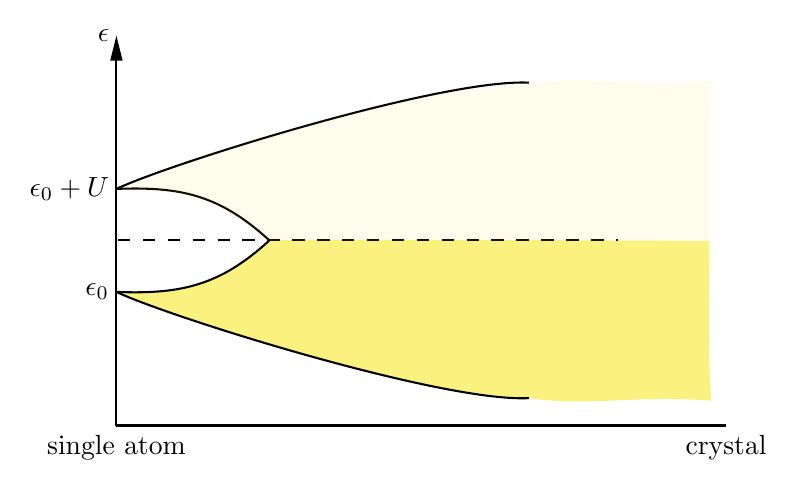
\begin{tikzpicture}[x=0.75pt,y=0.75pt,yscale=-1,xscale=1]
%uncomment if require: \path (0,300); %set diagram left start at 0, and has height of 300

%Shape: Polygon Curved [id:ds7075624570459664] 
\draw  [draw opacity=0][fill={rgb, 255:red, 248; green, 231; blue, 28 }  ,fill opacity=0.57 ] (173,213.63) .. controls (198.71,216.07) and (226.71,209.07) .. (246.71,188.81) .. controls (296.71,188.07) and (439.71,189.07) .. (458.71,189.07) .. controls (458.71,210.07) and (457.71,245.07) .. (459.71,266.07) .. controls (422.71,263.07) and (401.71,269.07) .. (371.71,264.81) .. controls (315.71,262.07) and (231.71,237.07) .. (173,213.63) -- cycle ;
%Straight Lines [id:da8100808760339464] 
\draw    (173,278) -- (466.71,278) ;
%Straight Lines [id:da1730446730702535] 
\draw    (173,92.19) -- (173,278) ;
\draw [shift={(173,90.19)}, rotate = 90] [fill={rgb, 255:red, 0; green, 0; blue, 0 }  ][line width=0.08]  [draw opacity=0] (12,-3) -- (0,0) -- (12,3) -- cycle    ;
%Curve Lines [id:da37288245167395306] 
\draw    (173,164) .. controls (203.71,162.81) and (222.71,166.81) .. (246.71,188.81) ;
%Curve Lines [id:da1329203045652183] 
\draw    (173,213.63) .. controls (203.71,214.81) and (222.71,210.81) .. (246.71,188.81) ;
%Curve Lines [id:da9577944633435271] 
\draw    (173,164) .. controls (198.71,151.81) and (329.71,110.81) .. (371.71,112.81) ;
%Curve Lines [id:da3428932734540302] 
\draw    (173,213.63) .. controls (198.71,225.81) and (329.71,266.81) .. (371.71,264.81) ;
%Straight Lines [id:da604449076641173] 
\draw  [dash pattern={on 4.5pt off 4.5pt}]  (173.71,188.81) -- (414.71,188.81) ;
%Shape: Polygon Curved [id:ds33698675422401303] 
\draw  [draw opacity=0][fill={rgb, 255:red, 248; green, 231; blue, 28 }  ,fill opacity=0.08 ] (173,164.52) .. controls (198.71,162.07) and (226.71,169.07) .. (246.71,189.33) .. controls (296.71,190.07) and (439.71,189.07) .. (458.71,189.07) .. controls (458.71,168.07) and (457.71,133.07) .. (459.71,112.07) .. controls (422.71,115.07) and (401.71,109.07) .. (371.71,113.33) .. controls (315.71,116.07) and (231.71,141.07) .. (173,164.52) -- cycle ;

% Text Node
\draw (173,281) node [anchor=north] [inner sep=0.75pt]   [align=left] {single atom};
% Text Node
\draw (466.71,281) node [anchor=north] [inner sep=0.75pt]   [align=left] {crystal};
% Text Node
\draw (171,90.19) node [anchor=east] [inner sep=0.75pt]    {$\epsilon $};
% Text Node
\draw (171,213.63) node [anchor=east] [inner sep=0.75pt]    {$\epsilon _{0}$};
% Text Node
\draw (171,164) node [anchor=east] [inner sep=0.75pt]    {$\epsilon _{0} +U$};


\end{tikzpicture}

    \caption{电子-电子排斥导致的能带撕裂,黄色区域表示有能级的区域}
    \label{fig:mott-band}
\end{figure}

以上物理图像意味着,对局域电子,on-site interaction能够造成与巡游电子的能带理论非常不同的行为,形象地说就是“能带撕裂”:如\autoref{fig:mott-band}所示,在原子间隔较大,单个原子可以看成孤立原子的极限下(\autoref{fig:mott-band}最左边),由于on-site repulsion,可以认为同一个轨道上的两个电子的能量因为库伦排斥而取消简并,表示为$\epsilon_0$和$\epsilon_0 + U$两个能级。
由于晶体中有$N$个原子,这两个能级均高度简并,各有$N$重简并。
随着原子间距拉近,原子中的电子感受到由弱到强的周期势场,能级取消简并而形成能带(\autoref{fig:mott-band}中体现为$\epsilon_0$和$\epsilon_0 + U$均“变宽了”)。
在原子间距不很近时,有两条能带,中间隔了一个能隙。
如果系统中共有$N$个电子,那么从下往上填充能带,会发现一条能带全满(\autoref{fig:mott-band}中标为深黄色),而另一条能带全空(\autoref{fig:mott-band}中标为浅黄色),从而系统是绝缘体。
而当两条能带发生交叠时,系统就成了导体。
因此,一个由一价原子形成的晶体电子跃迁能力相对于on-site repulsion小时为绝缘体而电子跃迁能力相对于on-site repulsion大时为导体。

\subsection{Hubbard模型}

我们注意到Hubbard相互作用是on-site repulsion,从而,如下\concept{Hubbard模型}
\begin{equation}
    H = - t \sum_{\pair{\vb*{i}, \vb*{j}}, \alpha} c^\dagger_{\vb*{i} \alpha} c_{\vb*{j} \alpha} - \mu N + U \sum_{\vb*{i}} n_{\vb*{i} \uparrow} n_{\vb*{i} \downarrow}
\end{equation}
很可能是Mott绝缘体的一个例子。



\subsection{海森堡模型和t-J模型}

我们尚没有讨论Hubbard模型的Mott绝缘体基态附近的理论是什么样的。基本的自由度肯定不是能带导体中的载流子——实际上我们将看到,半满Hubbard模型(即$\mu=0$的情况)的Mott态附近的模型是海森堡模型,稍微偏离半满的情况对应t-J模型。

先分析半满Hubbard模型。$U \gg t$的情况下哈密顿量为
\[
    H = U \sum_{\vb*{i}} n_{\vb*{i} \uparrow} n_{\vb*{i} \downarrow},
\]
由于是半满Hubbard模型,系统基态是可以很容易确定的:每个格点上要么有一个自旋向上的电子,要么有一个自旋向下的电子。
所有这些状态的能量都精确是$0$。由于$U$非常大,一个有一个格点上有两个电子的状态一定是非常高能的,因此我们可以有把握地说:系统的低能子空间是每个格点上一个电子的那部分态矢量组成的希尔伯特空间。

\begin{figure}
    \centering
    \subfigure[如果相邻的$\vb*{i}$格点和$\vb*{j}$上的电子自旋平行,则它们之间不存在有效相互作用通道]{
        

\tikzset{every picture/.style={line width=0.75pt}} %set default line width to 0.75pt        

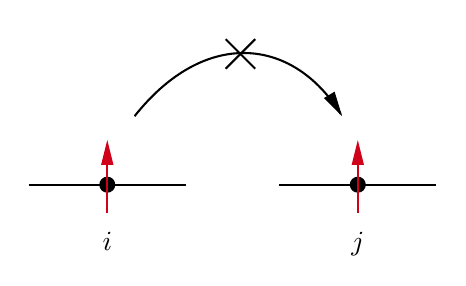
\begin{tikzpicture}[x=0.75pt,y=0.75pt,yscale=-1,xscale=1]
%uncomment if require: \path (0,300); %set diagram left start at 0, and has height of 300

%Straight Lines [id:da7386552192639442] 
\draw    (82,149) -- (157.71,149) ;
%Straight Lines [id:da9226927043104383] 
\draw    (202.71,149) -- (278.41,149) ;
%Straight Lines [id:da04346239197026791] 
\draw    (119.85,149) ;
\draw [shift={(119.85,149)}, rotate = 0] [color={rgb, 255:red, 0; green, 0; blue, 0 }  ][fill={rgb, 255:red, 0; green, 0; blue, 0 }  ][line width=0.75]      (0, 0) circle [x radius= 3.35, y radius= 3.35]   ;
%Straight Lines [id:da49104348516978225] 
\draw    (240.56,149) ;
\draw [shift={(240.56,149)}, rotate = 0] [color={rgb, 255:red, 0; green, 0; blue, 0 }  ][fill={rgb, 255:red, 0; green, 0; blue, 0 }  ][line width=0.75]      (0, 0) circle [x radius= 3.35, y radius= 3.35]   ;
%Straight Lines [id:da7990616031157829] 
\draw [color={rgb, 255:red, 208; green, 2; blue, 27 }  ,draw opacity=1 ]   (119.85,162.5) -- (119.85,129.5) ;
\draw [shift={(119.85,127.5)}, rotate = 450] [fill={rgb, 255:red, 208; green, 2; blue, 27 }  ,fill opacity=1 ][line width=0.08]  [draw opacity=0] (12,-3) -- (0,0) -- (12,3) -- cycle    ;
%Straight Lines [id:da17695895554295893] 
\draw [color={rgb, 255:red, 208; green, 2; blue, 27 }  ,draw opacity=1 ]   (240.56,162.5) -- (240.56,129.5) ;
\draw [shift={(240.56,127.5)}, rotate = 450] [fill={rgb, 255:red, 208; green, 2; blue, 27 }  ,fill opacity=1 ][line width=0.08]  [draw opacity=0] (12,-3) -- (0,0) -- (12,3) -- cycle    ;
%Curve Lines [id:da9848910002402611] 
\draw    (133,116) .. controls (166.37,73.85) and (208.85,77.35) .. (232.3,114.85) ;
\draw [shift={(233,116)}, rotate = 238.87] [fill={rgb, 255:red, 0; green, 0; blue, 0 }  ][line width=0.08]  [draw opacity=0] (12,-3) -- (0,0) -- (12,3) -- cycle    ;
%Straight Lines [id:da5300373220437029] 
\draw    (184,86) ;
\draw [shift={(184,86)}, rotate = 45] [color={rgb, 255:red, 0; green, 0; blue, 0 }  ][line width=0.75]    (-10.06,0) -- (10.06,0)(0,10.06) -- (0,-10.06)   ;

% Text Node
\draw (119.85,170.4) node [anchor=north] [inner sep=0.75pt]    {$\boldsymbol{i}$};
% Text Node
\draw (240.56,170.4) node [anchor=north] [inner sep=0.75pt]    {$\boldsymbol{j}$};


\end{tikzpicture}

        \label{fig:hubbard-effective-interaction-pauli-exclusive}
    }
    \subfigure[如果相邻的$\vb*{i}$格点和$\vb*{j}$上的电子自旋反平行,则它们之间存在有效相互作用通道:存在一个电子跑到另一个格点上,然后另一个电子跑回来的过程]{
        

\tikzset{every picture/.style={line width=0.75pt}} %set default line width to 0.75pt        

\begin{tikzpicture}[x=0.75pt,y=0.75pt,yscale=-1,xscale=1]
%uncomment if require: \path (0,300); %set diagram left start at 0, and has height of 300

%Straight Lines [id:da20191335231513108] 
\draw    (61,208) -- (136.71,208) ;
%Straight Lines [id:da3306943554899906] 
\draw    (145.71,208) -- (221.41,208) ;
%Straight Lines [id:da0476257107983713] 
\draw    (98.85,208) ;
\draw [shift={(98.85,208)}, rotate = 0] [color={rgb, 255:red, 0; green, 0; blue, 0 }  ][fill={rgb, 255:red, 0; green, 0; blue, 0 }  ][line width=0.75]      (0, 0) circle [x radius= 3.35, y radius= 3.35]   ;
%Straight Lines [id:da810233186905045] 
\draw    (183.56,208) ;
\draw [shift={(183.56,208)}, rotate = 0] [color={rgb, 255:red, 0; green, 0; blue, 0 }  ][fill={rgb, 255:red, 0; green, 0; blue, 0 }  ][line width=0.75]      (0, 0) circle [x radius= 3.35, y radius= 3.35]   ;
%Straight Lines [id:da5292766411522429] 
\draw [color={rgb, 255:red, 208; green, 2; blue, 27 }  ,draw opacity=1 ]   (98.85,221.5) -- (98.85,188.5) ;
\draw [shift={(98.85,186.5)}, rotate = 450] [fill={rgb, 255:red, 208; green, 2; blue, 27 }  ,fill opacity=1 ][line width=0.08]  [draw opacity=0] (12,-3) -- (0,0) -- (12,3) -- cycle    ;
%Straight Lines [id:da16952209334741952] 
\draw [color={rgb, 255:red, 74; green, 144; blue, 226 }  ,draw opacity=1 ]   (183.56,190.5) -- (183.56,223.5) ;
\draw [shift={(183.56,225.5)}, rotate = 270] [fill={rgb, 255:red, 74; green, 144; blue, 226 }  ,fill opacity=1 ][line width=0.08]  [draw opacity=0] (12,-3) -- (0,0) -- (12,3) -- cycle    ;
%Straight Lines [id:da8473032189254806] 
\draw    (457,209) -- (532.71,209) ;
%Straight Lines [id:da26615967357291437] 
\draw    (541.71,209) -- (617.41,209) ;
%Straight Lines [id:da9617695114523024] 
\draw    (494.85,209) ;
\draw [shift={(494.85,209)}, rotate = 0] [color={rgb, 255:red, 0; green, 0; blue, 0 }  ][fill={rgb, 255:red, 0; green, 0; blue, 0 }  ][line width=0.75]      (0, 0) circle [x radius= 3.35, y radius= 3.35]   ;
%Straight Lines [id:da9166380580229472] 
\draw    (579.56,209) ;
\draw [shift={(579.56,209)}, rotate = 0] [color={rgb, 255:red, 0; green, 0; blue, 0 }  ][fill={rgb, 255:red, 0; green, 0; blue, 0 }  ][line width=0.75]      (0, 0) circle [x radius= 3.35, y radius= 3.35]   ;
%Straight Lines [id:da90841483514599] 
\draw [color={rgb, 255:red, 208; green, 2; blue, 27 }  ,draw opacity=1 ]   (579.56,222.5) -- (579.56,189.5) ;
\draw [shift={(579.56,187.5)}, rotate = 450] [fill={rgb, 255:red, 208; green, 2; blue, 27 }  ,fill opacity=1 ][line width=0.08]  [draw opacity=0] (12,-3) -- (0,0) -- (12,3) -- cycle    ;
%Straight Lines [id:da5212507878125441] 
\draw [color={rgb, 255:red, 74; green, 144; blue, 226 }  ,draw opacity=1 ]   (494.85,192.5) -- (494.85,225.5) ;
\draw [shift={(494.85,227.5)}, rotate = 270] [fill={rgb, 255:red, 74; green, 144; blue, 226 }  ,fill opacity=1 ][line width=0.08]  [draw opacity=0] (12,-3) -- (0,0) -- (12,3) -- cycle    ;
%Straight Lines [id:da7686303558967333] 
\draw    (254,75) -- (329.71,75) ;
%Straight Lines [id:da39580118305367007] 
\draw    (338.71,75) -- (414.41,75) ;
%Straight Lines [id:da9698766463324444] 
\draw    (393.56,75) ;
\draw [shift={(393.56,75)}, rotate = 0] [color={rgb, 255:red, 0; green, 0; blue, 0 }  ][fill={rgb, 255:red, 0; green, 0; blue, 0 }  ][line width=0.75]      (0, 0) circle [x radius= 3.35, y radius= 3.35]   ;
%Straight Lines [id:da3017208196262404] 
\draw [color={rgb, 255:red, 74; green, 144; blue, 226 }  ,draw opacity=1 ]   (393.56,57.5) -- (393.56,90.5) ;
\draw [shift={(393.56,92.5)}, rotate = 270] [fill={rgb, 255:red, 74; green, 144; blue, 226 }  ,fill opacity=1 ][line width=0.08]  [draw opacity=0] (12,-3) -- (0,0) -- (12,3) -- cycle    ;
%Straight Lines [id:da270365844915331] 
\draw    (358.85,75) ;
\draw [shift={(358.85,75)}, rotate = 0] [color={rgb, 255:red, 0; green, 0; blue, 0 }  ][fill={rgb, 255:red, 0; green, 0; blue, 0 }  ][line width=0.75]      (0, 0) circle [x radius= 3.35, y radius= 3.35]   ;
%Straight Lines [id:da9878568474884404] 
\draw [color={rgb, 255:red, 208; green, 2; blue, 27 }  ,draw opacity=1 ]   (358.85,88.5) -- (358.85,55.5) ;
\draw [shift={(358.85,53.5)}, rotate = 450] [fill={rgb, 255:red, 208; green, 2; blue, 27 }  ,fill opacity=1 ][line width=0.08]  [draw opacity=0] (12,-3) -- (0,0) -- (12,3) -- cycle    ;
%Straight Lines [id:da43506871848231543] 
\draw    (135.71,168.19) -- (219.32,81.63) ;
\draw [shift={(220.71,80.19)}, rotate = 494.01] [fill={rgb, 255:red, 0; green, 0; blue, 0 }  ][line width=0.08]  [draw opacity=0] (12,-3) -- (0,0) -- (12,3) -- cycle    ;
%Straight Lines [id:da5330814497610539] 
\draw    (531.32,166.75) -- (447.71,80.19) ;
\draw [shift={(532.71,168.19)}, rotate = 225.99] [fill={rgb, 255:red, 0; green, 0; blue, 0 }  ][line width=0.08]  [draw opacity=0] (12,-3) -- (0,0) -- (12,3) -- cycle    ;

% Text Node
\draw (98.85,229.4) node [anchor=north] [inner sep=0.75pt]    {$\boldsymbol{i}$};
% Text Node
\draw (183.56,229.4) node [anchor=north] [inner sep=0.75pt]    {$\boldsymbol{j}$};
% Text Node
\draw (494.85,230.4) node [anchor=north] [inner sep=0.75pt]    {$\boldsymbol{i}$};
% Text Node
\draw (579.56,230.4) node [anchor=north] [inner sep=0.75pt]    {$\boldsymbol{j}$};
% Text Node
\draw (291.85,96.4) node [anchor=north] [inner sep=0.75pt]    {$\boldsymbol{i}$};
% Text Node
\draw (376.56,96.4) node [anchor=north] [inner sep=0.75pt]    {$\boldsymbol{j}$};


\end{tikzpicture}

    }
    \caption{紧束缚跃迁项导致的有效相互作用通道}
    \label{fig:effective-spin-interaction-hubbard}
\end{figure}

现在我们将跃迁项作为微扰加入回去。如\autoref{fig:effective-spin-interaction-hubbard}所示,低能子空间中的每一个状态都是零,而两个电子挤在一个格点上的状态能量为$U$,于是我们有等效相互作用
\[
    \sum_{\pair{\vb*{i}, \vb*{j}}, \alpha, \beta} (-t c^\dagger_{\vb*{i} \alpha} c_{\vb*{j} \alpha}) \frac{1}{0 - U} (-t c^\dagger_{\vb*{j} \beta} c_{\vb*{i} \beta}) = - \frac{t^2}{U} \sum_{\pair{\vb*{i}, \vb*{j}}, \alpha, \beta} c^\dagger_{\vb*{i} \alpha} c_{\vb*{j} \alpha} c^\dagger_{\vb*{j} \beta} c_{\vb*{i} \beta}.
\]
注意这个等效相互作用的形式已经自动地将泡利不相容原理考虑在内了,从而\autoref{fig:hubbard-effective-interaction-pauli-exclusive}展示的不可能性已经被满足了。
根据\eqref{eq:pauli-dot-product}有


这就是说,在半满Hubbard模型中,低能激发中只有自旋自由度而没有电荷自由度。

从Hubbard模型产生出了海森堡模型是多少有些令人惊奇的,因为Hubbard模型中来自库伦排斥的$n_\uparrow n_\downarrow$项表面上看\emph{不能}提供交换两个电子的相互作用通道,似乎无法产生任何自旋-自旋相互作用。
然而,跃迁项的存在让我们能够通过一些中间步骤产生电子交换和交换相互作用。

\begin{equation}
    H = - t \sum_{\vb*{i}, \alpha} (c_{\vb*{i} \alpha}^\dagger c_{\vb*{j} \alpha} + \text{h.c.}) + \sum_{\pair{\vb*{i}, \vb*{j}}} J \vb*{S}_{\vb*{i}} \cdot \vb*{S}_{\vb*{j}}
\end{equation}

Goodenough规则:如果电子跃迁是在两个半满轨道之间,那么就是反铁磁序,如果电子跃迁是从一个半满轨道到一个空轨道,或是从一个全满轨道到一个半满轨道,那么就是铁磁序。

\section{Wigner晶体}

% TODO:电子晶体,以及它和DFT计算之间的关系